\documentclass{article}%
\usepackage[T1]{fontenc}%
\usepackage[utf8]{inputenc}%
\usepackage{lmodern}%
\usepackage{textcomp}%
\usepackage{lastpage}%
\usepackage{geometry}%
\geometry{margin=1in,headheight=14pt,headsep=25pt}%
\usepackage{hyperref}%
\usepackage{enumitem}%
\usepackage{fancyhdr}%
\usepackage{xcolor}%
\usepackage{url}%
\usepackage{breakurl}%
\usepackage{amsmath}%
\usepackage{amssymb}%
\usepackage{mathtools}%
\usepackage{amsthm}%
\usepackage{thmtools}%
\usepackage{float}%
\usepackage{subcaption}%
\usepackage[font=small,labelfont=bf]{caption}%
%

            \hypersetup{
                colorlinks=true,
                linkcolor=blue,
                filecolor=magenta,
                urlcolor=blue,
                breaklinks=true,
                bookmarks=true,
                pdfborder={0 0 0}
            }
            \urlstyle{same}
            \Urlmuskip=0mu plus 1mu  % URL breaking in nicer spots

            % Math configuration
            \everymath{\displaystyle}
            \setlength{\jot}{10pt}  % Increase spacing between equations

            \pagestyle{fancy}
            \fancyhf{}
            \rhead{Generated on \today}
            \cfoot{\thepage}

            % Better Unicode support
            \usepackage[utf8]{inputenc}
            \usepackage{newunicodechar}
            \setlength{\itemsep}{1em} % Adds spacing between items

            % Configure itemize settings globally
            \setlist[itemize]{nosep}
            \setlist[itemize]{leftmargin=*}

            % Remove section numbering
            \renewcommand{\thesection}{}
            \renewcommand{\thesubsection}{}

            % Adjust caption spacing around figures
            \setlength{\abovecaptionskip}{0pt}
            \setlength{\belowcaptionskip}{5pt}
        %
\lhead{Lecture: 07L2{-}Vision}%
\title{07L2{-}Vision}%
\author{Generated by Scribe.AI}%
\date{\today}%
%
\begin{document}%
\normalsize%
\maketitle%
\section{Slide 1}%
\label{sec:Slide1}%
\subsection{Content}%

\textbf{CS 24300 - AI Basics} \\
Tony Bergstrom \\
Slides adapted from Yexiang Xue
%
\subsection{Description}%
This slide is a title slide for a lecture on Artificial Intelligence Basics, likely part of a course called CS 24300.  It displays the course title, the instructor's name (Tony Bergstrom), and a credit line indicating that the slides are adapted from another source (Yexiang Xue).  There is no mathematical content on this slide.%
\subsection{Figures}%
\begin{figure}[H]%
\centering%
\end{figure}

%
\newpage%
\section{Slide 2}%
\label{sec:Slide2}%
\subsection{Content}%

Image Classification
%
\subsection{Description}%
This slide displays a single line of text: "Image Classification".  It is likely a title slide or a heading for a section within a presentation or lecture on Artificial Intelligence Basics, specifically focusing on a topic related to image recognition or image analysis.%
\subsection{Figures}%
\begin{figure}[H]%
\centering%
\end{figure}

%
\newpage%
\section{Slide 3}%
\label{sec:Slide3}%
\subsection{Content}%
%
\subsection{Description}%
This slide, titled "Image Classification," presents a basic concept in image recognition.  It shows an image of a gray tabby cat.  An arrow points from the image to the word "cat," indicating that the image is labeled as a "cat."  Below the image and arrow, the slide states "Assume given set of discrete labels {dog, cat, truck, plane, ...}". This implies that the system being discussed is designed to classify images into predefined categories, such as "cat," "dog," "truck," and so on.  The text also includes a credit line, "Part of this lecture is based on Fei-fei Li & Justin Johnson & Serena Yeung: CS231n at Stanford," indicating the source of the material. The context of the course (Artificial Intelligence Basics) suggests that this slide is introducing the fundamental idea of image classification as a task in AI.%
\subsection{Figures}%
\begin{figure}[H]%
\centering%
\begin{subfigure}[b]{0.15\textwidth}%
\centering%

\includegraphics[width=\textwidth]{/Users/ashoksaravanan/Coding/ScribeLec/server/output/CS 243/lectures/07L2-Vision/figures/3.1.png}%
\caption{}%
\end{subfigure}%
\end{figure}

%
\newpage%
\section{Slide 4}%
\label{sec:Slide4}%
\subsection{Content}%

\textbf{The Problem: Semantic Gap} \\
\textbf{What a computer "sees"} \\
An image is a big grid of numbers \\
between 0 and 255. \\
Each value represents Red, Green, or \\
Blue for a pixel \\
An 800 $\times$ 600 image is 800 $\times$ 600 $\times$ 3 \\
values: 1,440,000
%
\subsection{Description}%
This slide, part of a lecture on Artificial Intelligence Basics, discusses the "Semantic Gap" problem in image recognition.  It explains how a computer interprets an image.  The slide states that an image is represented as a grid of numbers, each between 0 and 255.  These numbers correspond to the intensity values of Red, Green, and Blue (RGB) color components for each pixel.  An 800x600 image, therefore, contains 1,440,000 such values.  The slide highlights the contrast between this numerical representation (what a computer "sees") and the human understanding of the image's content (the semantic meaning).  The image of a gray tabby cat is included to illustrate the concept.  The text "The Problem: Semantic Gap" indicates that the slide is introducing a key challenge in computer vision, namely the difficulty in translating the raw pixel data into meaningful interpretations.%
\subsection{Figures}%
\begin{figure}[H]%
\centering%
\begin{subfigure}[b]{0.15\textwidth}%
\centering%

\includegraphics[width=\textwidth]{/Users/ashoksaravanan/Coding/ScribeLec/server/output/CS 243/lectures/07L2-Vision/figures/4.1.png}%
\caption{}%
\end{subfigure}%
\hspace{0.05\textwidth}%
\begin{subfigure}[b]{0.15\textwidth}%
\centering%

\includegraphics[width=\textwidth]{/Users/ashoksaravanan/Coding/ScribeLec/server/output/CS 243/lectures/07L2-Vision/figures/4.2.png}%
\caption{}%
\end{subfigure}%
\end{figure}

%
\newpage%
\section{Slide 5}%
\label{sec:Slide5}%
\subsection{Content}%

Fit a HUGE logistic regression model? \\
Flatten the image matrix into a vector: \\
$I_{img} = \begin{bmatrix} a_{11} \\ \vdots \\ a_{1n} \\ \vdots \\ a_{m1} \\ \vdots \\ a_{mn} \end{bmatrix} \implies I_v = (a_{11}, \dots, a_{1n}, \dots, a_{m1}, \dots, a_{mn})^T$ \\
Fit a logistic regression model with $I_v$, as input: \\
prediction = sign($w^T I_v$) = sign$(\sum_{i,j} w_{i,j} a_{i,j})$ \\
Is this a good idea? What may be its problems?
%
\subsection{Description}%
This slide, part of a lecture on Artificial Intelligence Basics, discusses a potential approach to image classification using a logistic regression model.  It proposes flattening an image matrix ($I_{img}$) into a vector ($I_v$).  The image matrix is represented by $a_{i,j}$ where $i$ represents the row and $j$ represents the column.  The flattened vector $I_v$ contains all the elements of the image matrix in a single row.  The slide then suggests fitting a logistic regression model using this flattened vector as input.  The prediction is calculated as the sign of the dot product of the weight vector ($w$) and the flattened image vector ($I_v$).  The slide concludes with a question about the effectiveness and potential drawbacks of this approach.  The context of the course suggests that the slide is exploring different methods for image classification and evaluating their potential strengths and weaknesses.%
\subsection{Figures}%
\begin{figure}[H]%
\centering%
\end{figure}

%
\newpage%
\section{Slide 6}%
\label{sec:Slide6}%
\subsection{Content}%
%
\subsection{Description}%
%
\subsection{Figures}%
\begin{figure}[H]%
\centering%
\begin{subfigure}[b]{0.15\textwidth}%
\centering%

\includegraphics[width=\textwidth]{/Users/ashoksaravanan/Coding/ScribeLec/server/output/CS 243/lectures/07L2-Vision/figures/6.1.png}%
\caption{}%
\end{subfigure}%
\hspace{0.05\textwidth}%
\begin{subfigure}[b]{0.15\textwidth}%
\centering%

\includegraphics[width=\textwidth]{/Users/ashoksaravanan/Coding/ScribeLec/server/output/CS 243/lectures/07L2-Vision/figures/6.2.png}%
\caption{}%
\end{subfigure}%
\hspace{0.05\textwidth}%
\begin{subfigure}[b]{0.15\textwidth}%
\centering%

\includegraphics[width=\textwidth]{/Users/ashoksaravanan/Coding/ScribeLec/server/output/CS 243/lectures/07L2-Vision/figures/6.3.png}%
\caption{}%
\end{subfigure}%
\end{figure}

%
\newpage%
\section{Slide 7}%
\label{sec:Slide7}%
\subsection{Content}%

\textbf{Challenges: illumination}
%
\subsection{Description}%
This slide, part of a lecture on Artificial Intelligence Basics, focuses on the challenge of illumination in image recognition.  It displays three images of cats, each with different lighting conditions.  The first cat is in a dark setting, the second is in a setting with a strong light source highlighting its features, and the third is in a setting with dappled light and shadows.  The text "Challenges: illumination" indicates that the slide is introducing a specific problem in computer vision related to how varying light conditions can affect the way an image is perceived by a computer.  The images are likely examples to illustrate the difficulty of creating algorithms that can accurately interpret images regardless of the lighting conditions.  The text "This image is CC0 1.0 public domain" under each image indicates that the images are in the public domain and can be used freely.  The context of the course suggests that the slide is preparing to discuss techniques for dealing with variations in lighting when training image recognition models.%
\subsection{Figures}%
\begin{figure}[H]%
\centering%
\begin{subfigure}[b]{0.15\textwidth}%
\centering%

\includegraphics[width=\textwidth]{/Users/ashoksaravanan/Coding/ScribeLec/server/output/CS 243/lectures/07L2-Vision/figures/7.1.png}%
\caption{}%
\end{subfigure}%
\hspace{0.05\textwidth}%
\begin{subfigure}[b]{0.15\textwidth}%
\centering%

\includegraphics[width=\textwidth]{/Users/ashoksaravanan/Coding/ScribeLec/server/output/CS 243/lectures/07L2-Vision/figures/7.2.png}%
\caption{}%
\end{subfigure}%
\end{figure}

%
\newpage%
\section{Slide 8}%
\label{sec:Slide8}%
\subsection{Content}%

\textbf{Challenges: deformation}
%
\subsection{Description}%
This slide, part of a lecture on Artificial Intelligence Basics, highlights the "deformation" challenge in image recognition.  It presents four images of cats in different poses and orientations.  The images show variations in the cats' positions, suggesting that the same object (a cat) can appear differently in various orientations and poses.  The text "Challenges: deformation" indicates that the slide is introducing a specific problem in computer vision related to how variations in the shape and position of an object can affect the way an image is perceived by a computer.  The images are likely examples to illustrate the difficulty of creating algorithms that can accurately identify objects regardless of their pose or orientation.  The text under each image ("This image by [author] is licensed under CC-BY 2.0") indicates that the images are in the public domain and can be used freely.  The context of the course suggests that the slide is preparing to discuss techniques for dealing with variations in object pose and orientation when training image recognition models.%
\subsection{Figures}%
\begin{figure}[H]%
\centering%
\begin{subfigure}[b]{0.15\textwidth}%
\centering%

\includegraphics[width=\textwidth]{/Users/ashoksaravanan/Coding/ScribeLec/server/output/CS 243/lectures/07L2-Vision/figures/8.1.png}%
\caption{}%
\end{subfigure}%
\hspace{0.05\textwidth}%
\begin{subfigure}[b]{0.15\textwidth}%
\centering%

\includegraphics[width=\textwidth]{/Users/ashoksaravanan/Coding/ScribeLec/server/output/CS 243/lectures/07L2-Vision/figures/8.2.png}%
\caption{}%
\end{subfigure}%
\end{figure}

%
\newpage%
\section{Slide 9}%
\label{sec:Slide9}%
\subsection{Content}%

\textbf{Challenges: occlusion}
%
\subsection{Description}%
This slide, part of a lecture on Artificial Intelligence Basics, focuses on the challenge of "occlusion" in image recognition.  It displays three images of cats.  The first image shows a cat partially hidden under a blanket or cloth, illustrating how a portion of the object is obscured. The second image shows a cat partially hidden within tall grass, again demonstrating partial occlusion. The third image shows a cat lying on a couch, with part of its body hidden behind the couch's armrest.  The text "Challenges: occlusion" indicates that the slide is introducing a specific problem in computer vision related to how parts of an object might be hidden or obscured in an image.  The images are examples to illustrate the difficulty of creating algorithms that can accurately identify objects despite partial or complete occlusion.  The text under each image ("This image is CC0 1.0 public domain" or "This image by jonsson is licensed under CC-BY 2.0") indicates that the images are in the public domain or under a Creative Commons license and can be used freely.  The context of the course suggests that the slide is preparing to discuss techniques for dealing with occlusion when training image recognition models.%
\subsection{Figures}%
\begin{figure}[H]%
\centering%
\begin{subfigure}[b]{0.15\textwidth}%
\centering%

\includegraphics[width=\textwidth]{/Users/ashoksaravanan/Coding/ScribeLec/server/output/CS 243/lectures/07L2-Vision/figures/9.1.png}%
\caption{}%
\end{subfigure}%
\end{figure}

%
\newpage%
\section{Slide 10}%
\label{sec:Slide10}%
\subsection{Content}%

\textbf{Challenges: background clutter}
%
\subsection{Description}%
This slide, part of a lecture on Artificial Intelligence Basics, discusses the challenge of "background clutter" in image recognition.  It presents two images of cats. The first image shows a reddish-brown cat situated amidst fallen leaves and the ground. The second image shows a gray and white cat partially hidden within a snowy background with branches.  The text "Challenges: background clutter" indicates that the slide is introducing a specific problem in computer vision related to how distracting or irrelevant elements in the background of an image can affect the ability of an algorithm to identify the object of interest (the cat). The images are examples to illustrate the difficulty of creating algorithms that can accurately identify objects when the background is complex and contains similar colors or textures to the object itself. The text "This image is CC0 1.0 public domain" under each image indicates that the images are in the public domain and can be used freely. The context of the course suggests that the slide is preparing to discuss techniques for dealing with background clutter when training image recognition models.%
\subsection{Figures}%
\begin{figure}[H]%
\centering%
\begin{subfigure}[b]{0.15\textwidth}%
\centering%

\includegraphics[width=\textwidth]{/Users/ashoksaravanan/Coding/ScribeLec/server/output/CS 243/lectures/07L2-Vision/figures/10.1.png}%
\caption{}%
\end{subfigure}%
\end{figure}

%
\newpage%
\section{Slide 11}%
\label{sec:Slide11}%
\subsection{Content}%

\textbf{Image Classification}

Assume given set of discrete labels
\{dog, cat, truck, plane, ...\}

Need to find INVARIANT features
%
\subsection{Description}%
This slide, part of a lecture on Artificial Intelligence Basics, introduces the concept of image classification.  It states that a set of discrete labels (e.g., dog, cat, truck, plane) is given.  The key objective is to find "invariant features."  The slide likely precedes a discussion of techniques for extracting features from images that remain consistent regardless of variations in the image, such as changes in object position, size, or orientation.  A picture of a gray tabby cat is included, with the word "cat" below it and an arrow pointing to the word, indicating that the cat image is an example of the type of object being considered. The text "This image by Nikita is licensed under CC-BY 2.0" suggests the image is under a Creative Commons license. The context of the course suggests that the slide is introducing the problem of creating image recognition systems that can reliably identify objects despite variations in the image data.%
\subsection{Figures}%
\begin{figure}[H]%
\centering%
\begin{subfigure}[b]{0.15\textwidth}%
\centering%

\includegraphics[width=\textwidth]{/Users/ashoksaravanan/Coding/ScribeLec/server/output/CS 243/lectures/07L2-Vision/figures/11.1.png}%
\caption{}%
\end{subfigure}%
\end{figure}

%
\newpage%
\section{Slide 12}%
\label{sec:Slide12}%
\subsection{Content}%

\textbf{Bag of Features}
%
\subsection{Description}%
This slide, part of a lecture on Artificial Intelligence Basics, introduces the concept of a "Bag of Features."  The title, "Bag of Features," is presented in bold text.  The slide likely precedes a discussion of image representation techniques, specifically those that treat an image as a collection of features, disregarding the spatial relationships between them.  The context of the course suggests that this is a fundamental concept in image recognition and classification, where the focus shifts from the spatial arrangement of pixels to the presence and frequency of various features within the image.  The lack of any other content on the slide indicates that this is a simple title slide or a heading for a subsequent section, which will elaborate on the details of the Bag of Features approach.%
\subsection{Figures}%
\begin{figure}[H]%
\centering%
\end{figure}

%
\newpage%
\section{Slide 13}%
\label{sec:Slide13}%
\subsection{Content}%

\textbf{Key idea: classify based on invariant features!}

\textbf{Object} $\implies$ \textbf{Bag of 'words'}
%
\subsection{Description}%
This slide, part of a lecture on Artificial Intelligence Basics, introduces the concept of classifying objects based on invariant features.  It uses a visual metaphor to illustrate the "Bag of Words" approach.  On the left, an image of a portrait (likely a historical painting) is labeled "Object."  On the right, a paper bag is shown, with various small images (likely extracted features) of faces, or other visual elements, inside the bag.  This bag is labeled "Bag of 'words'."  The arrow connecting the two indicates that the object is represented by a collection of its constituent features, which are treated independently of their spatial arrangement.  The context of the course suggests that this slide is introducing a method for image classification where the algorithm focuses on the presence and frequency of certain visual features, rather than their precise location within the image.  The slide is likely preparing to discuss the details of the Bag of Features method, which is a common technique in computer vision for image classification.%
\subsection{Figures}%
\begin{figure}[H]%
\centering%
\begin{subfigure}[b]{0.15\textwidth}%
\centering%

\includegraphics[width=\textwidth]{/Users/ashoksaravanan/Coding/ScribeLec/server/output/CS 243/lectures/07L2-Vision/figures/13.1.png}%
\caption{}%
\end{subfigure}%
\hspace{0.05\textwidth}%
\begin{subfigure}[b]{0.15\textwidth}%
\centering%

\includegraphics[width=\textwidth]{/Users/ashoksaravanan/Coding/ScribeLec/server/output/CS 243/lectures/07L2-Vision/figures/13.2.png}%
\caption{}%
\end{subfigure}%
\end{figure}

%
\newpage%
\section{Slide 14}%
\label{sec:Slide14}%
\subsection{Content}%

\textbf{Visual words}
%
\subsection{Description}%
This slide, part of a lecture on Artificial Intelligence Basics, displays a set of images, each highlighting a specific visual feature.  The title "Visual words" is presented in bold text.  The images are arranged in rows and columns, likely representing different categories or types of visual features.  Each image shows a portion of an object (e.g., a human eye, a tire, or an airplane).  A yellow circle is drawn around a specific point within each image, with a small red dot inside the circle.  This suggests that the images are examples of "visual words" or "visual features" extracted from larger images.  The images are likely examples of features used in a "Bag of Features" approach to image classification.  The citation "[Sivic et al., ‘05]" at the bottom of the slide indicates that the visual words are based on work by Sivic et al. from 2005.  The context of the course suggests that the slide is illustrating a method for representing images as collections of visual features, which can then be used for tasks like image classification or retrieval.%
\subsection{Figures}%
\begin{figure}[H]%
\centering%
\begin{subfigure}[b]{0.15\textwidth}%
\centering%

\includegraphics[width=\textwidth]{/Users/ashoksaravanan/Coding/ScribeLec/server/output/CS 243/lectures/07L2-Vision/figures/14.1.png}%
\caption{}%
\end{subfigure}%
\end{figure}

%
\newpage%
\section{Slide 15}%
\label{sec:Slide15}%
\subsection{Content}%

\textbf{Object classification with bag of words}
%
\subsection{Description}%
This slide, part of a lecture on Artificial Intelligence Basics, displays the title "Object classification with bag of words."  Below the title, there are multiple small images arranged in a grid.  The images appear to be different indoor scenes, likely office or workspace environments.  Each scene shows various objects, including computers, bookshelves, and other furniture.  The images are likely examples of the types of images that would be used in a bag-of-words approach to object classification.  The citation "[Sivic et al., ‘05]" at the bottom of the slide indicates that the method is based on work by Sivic et al. from 2005.  The context of the course suggests that this slide is illustrating a method for classifying objects in images by analyzing the presence and frequency of visual features (visual words) within the image, rather than their spatial relationships.  The slide is likely preparing to discuss the details of the bag-of-words model for image classification.%
\subsection{Figures}%
\begin{figure}[H]%
\centering%
\begin{subfigure}[b]{0.15\textwidth}%
\centering%

\includegraphics[width=\textwidth]{/Users/ashoksaravanan/Coding/ScribeLec/server/output/CS 243/lectures/07L2-Vision/figures/15.1.png}%
\caption{}%
\end{subfigure}%
\hspace{0.05\textwidth}%
\begin{subfigure}[b]{0.15\textwidth}%
\centering%

\includegraphics[width=\textwidth]{/Users/ashoksaravanan/Coding/ScribeLec/server/output/CS 243/lectures/07L2-Vision/figures/15.2.png}%
\caption{}%
\end{subfigure}%
\end{figure}

%
\newpage%
\section{Slide 16}%
\label{sec:Slide16}%
\subsection{Content}%

\textbf{Bag of Features}

Represent images by frequencies of "visual words" (Bags of features)
%
\subsection{Description}%
This slide, part of a lecture on Artificial Intelligence Basics, introduces the "Bag of Features" method for image representation.  The title "Bag of Features" is displayed prominently.  Below the title, the slide describes the method as representing images by the frequencies of "visual words" (also referred to as "Bags of features").  The slide likely illustrates this concept with visual examples.  The context of the course suggests that this slide is introducing a method for image classification or retrieval where the algorithm focuses on the presence and frequency of certain visual features, rather than their precise location within the image.  The slide is likely to be followed by examples of how these features are extracted and used to represent images.  The slide shows two bar graphs, each representing the frequency of different visual features (visual words) in two different images.  The visual features are small images (e.g., an eye, a bicycle, a violin) that are likely extracted from the original images.  The height of each bar corresponds to the frequency of that particular visual word in the image.  The arrows indicate the direction of the image representation.  The context of the course is crucial for understanding the significance of this method in image analysis and classification tasks.%
\subsection{Figures}%
\begin{figure}[H]%
\centering%
\begin{subfigure}[b]{0.15\textwidth}%
\centering%

\includegraphics[width=\textwidth]{/Users/ashoksaravanan/Coding/ScribeLec/server/output/CS 243/lectures/07L2-Vision/figures/16.1.png}%
\caption{}%
\end{subfigure}%
\hspace{0.05\textwidth}%
\begin{subfigure}[b]{0.15\textwidth}%
\centering%

\includegraphics[width=\textwidth]{/Users/ashoksaravanan/Coding/ScribeLec/server/output/CS 243/lectures/07L2-Vision/figures/16.10.png}%
\caption{}%
\end{subfigure}%
\hspace{0.05\textwidth}%
\begin{subfigure}[b]{0.15\textwidth}%
\centering%

\includegraphics[width=\textwidth]{/Users/ashoksaravanan/Coding/ScribeLec/server/output/CS 243/lectures/07L2-Vision/figures/16.11.png}%
\caption{}%
\end{subfigure}%
\hspace{0.05\textwidth}%
\begin{subfigure}[b]{0.15\textwidth}%
\centering%

\includegraphics[width=\textwidth]{/Users/ashoksaravanan/Coding/ScribeLec/server/output/CS 243/lectures/07L2-Vision/figures/16.12.png}%
\caption{}%
\end{subfigure}%
\hspace{0.05\textwidth}%
\begin{subfigure}[b]{0.15\textwidth}%
\centering%

\includegraphics[width=\textwidth]{/Users/ashoksaravanan/Coding/ScribeLec/server/output/CS 243/lectures/07L2-Vision/figures/16.13.png}%
\caption{}%
\end{subfigure}%
\end{figure}

%
\newpage%
\section{Slide 17}%
\label{sec:Slide17}%
\subsection{Content}%

\textbf{Bag of Features (continued)}
%
\subsection{Description}%
This slide, part of a lecture on Artificial Intelligence Basics, continues the discussion of the Bag of Features method for image representation.  The title "Bag of Features (continued)" indicates a continuation of the previous slide's topic.  The slide displays a histogram (a bar graph) where the x-axis represents "codewords" (visual words) and the y-axis represents "frequency."  The bars are colored light pink, indicating the frequency of each codeword.  The codewords are represented by small grayscale images, likely visual features extracted from images.  A grayscale image of a street scene, likely a traffic scene, is shown in the upper right corner of the slide.  Red and green squares are drawn on the image, likely highlighting specific codewords or visual features that are present in the image.  The frequency of each codeword in the histogram corresponds to the presence of that feature in the image.  The context of the course suggests that the slide is illustrating how the Bag of Features method represents an image by counting the occurrences of various visual features.  The red and green squares on the image, along with the corresponding bars in the histogram, visually demonstrate the concept of feature frequency representation.  The slide is likely part of a discussion on image classification or retrieval using the Bag of Features approach.%
\subsection{Figures}%
\begin{figure}[H]%
\centering%
\begin{subfigure}[b]{0.15\textwidth}%
\centering%

\includegraphics[width=\textwidth]{/Users/ashoksaravanan/Coding/ScribeLec/server/output/CS 243/lectures/07L2-Vision/figures/17.1.png}%
\caption{}%
\end{subfigure}%
\end{figure}

%
\newpage%
\section{Slide 18}%
\label{sec:Slide18}%
\subsection{Content}%

\textbf{Bag of Features Object Categorization}

How do we use Bag of Features for object categorization?

\textbf{category models} \quad \quad \textbf{Model space}

\begin{tikzpicture}
  % Category models
  \foreach \i in {1,2,3} {
    \begin{axis}[
      width=4cm,
      height=3cm,
      xlabel=Codewords,
      ylabel=Frequency,
      xmin=0, xmax=10,
      ymin=0, ymax=10,
      xtick=\empty,
      ytick=\empty,
      title=Class \i,
      axis lines=left,
    ]
    \addplot+[ybar, fill=teal!60] coordinates {(1, 2) (2, 5) (3, 3) (4, 7) (5, 2) (6, 4) (7, 6) (8, 3) (9, 1) (10, 5)};
    \end{axis}
  }
  \node[below=0.5cm of axis cs:5,5] {$\dots$};
  \begin{axis}[
      width=4cm,
      height=3cm,
      xlabel=Codewords,
      ylabel=Frequency,
      xmin=0, xmax=10,
      ymin=0, ymax=10,
      xtick=\empty,
      ytick=\empty,
      title=Class N,
      axis lines=left,
    ]
    \addplot+[ybar, fill=magenta!60] coordinates {(1, 2) (2, 1) (3, 8) (4, 4) (5, 6) (6, 2) (7, 3) (8, 7) (9, 9) (10, 1)};
    \end{axis}
  }

  % Model space
  \begin{axis}[
    width=4cm,
    height=3cm,
    xlabel=Dimension 1,
    ylabel=Dimension 2,
    zlabel=Dimension 3,
    xmin=-2, xmax=2,
    ymin=-2, ymax=2,
    zmin=-2, zmax=2,
    axis lines=middle,
    view={60}{30},
  ]
  \addplot3[only marks, mark=*, mark size=3pt, blue] coordinates {(1, 1, 1) (1.5, 1.5, 1.5)};
  \addplot3[only marks, mark=*, mark size=3pt, magenta] coordinates {(1.5, -1, -1) (-1, 1, 1)};
  \end{axis}
\end{tikzpicture}

Class 1 \quad Class N
%
\subsection{Description}%
This slide, part of a lecture on Artificial Intelligence Basics, discusses object categorization using the Bag of Features method.  The title "Bag of Features Object Categorization" is displayed.  The slide then asks "How do we use Bag of Features for object categorization?".  The slide shows a visual representation of the method.  On the left side, there are multiple bar graphs, each representing a "category model" for a different class (e.g., Class 1, Class N).  Each bar graph displays the frequency of different "codewords" (visual features) within an image.  The x-axis represents the codewords, and the y-axis represents the frequency.  The bars are colored differently for each class, likely to visually distinguish the different categories.  The bars' heights represent the frequency of each codeword in the image.  The slide also shows a 3D scatter plot on the right, labeled "Model space."  The points in the scatter plot represent the category models in a multi-dimensional space.  The points are colored differently, likely corresponding to the different classes.  The context of the course suggests that this slide is illustrating how the Bag of Features method represents images as a collection of visual features and how these representations can be used to categorize objects by comparing them to pre-defined category models in a multi-dimensional space.  The slide is likely to be followed by a discussion of how to use these category models for classification.%
\subsection{Figures}%
\begin{figure}[H]%
\centering%
\begin{subfigure}[b]{0.15\textwidth}%
\centering%

\includegraphics[width=\textwidth]{/Users/ashoksaravanan/Coding/ScribeLec/server/output/CS 243/lectures/07L2-Vision/figures/18.1.png}%
\caption{}%
\end{subfigure}%
\end{figure}

%
\newpage%
\section{Slide 19}%
\label{sec:Slide19}%
\subsection{Content}%
%
\subsection{Description}%
This slide, part of a lecture on Artificial Intelligence Basics, discusses a key idea for object classification: using invariant features.  The title "Key idea: classify based on invariant features!" is displayed.  A diagram illustrates the process.  An image of an object (likely a portrait) is shown on the left, labeled "Object."  An arrow points from the object to a rectangular box labeled "Feature vector $f$."  This box represents a vector of features extracted from the image.  Below the box, there are arrows pointing down from the box to different feature components.  The features are explicitly listed as "#eyes" and "Mouth below eyes."  There are also ellipses (...), indicating other features that are not explicitly shown.  An arrow points down from the feature vector to the text "Fit logistic regression model."  Finally, the text "prediction = sign($w \cdot f$)" indicates that a logistic regression model is used to calculate a prediction based on the dot product of a weight vector $w$ and the feature vector $f$.  The context suggests that the slide is introducing a method for object recognition that focuses on identifying invariant features, such as the presence of eyes and the position of the mouth, regardless of the object's pose or scale.  The use of logistic regression implies a binary classification task (e.g., is it a face or not?).%
\subsection{Figures}%
\begin{figure}[H]%
\centering%
\begin{subfigure}[b]{0.15\textwidth}%
\centering%

\includegraphics[width=\textwidth]{/Users/ashoksaravanan/Coding/ScribeLec/server/output/CS 243/lectures/07L2-Vision/figures/19.1.png}%
\caption{}%
\end{subfigure}%
\end{figure}

%
\newpage%
\section{Slide 20}%
\label{sec:Slide20}%
\subsection{Content}%
%
\subsection{Description}%
This slide, part of a lecture on Artificial Intelligence Basics, focuses on document retrieval.  It shows a visual representation of word frequencies from various documents.  The slide displays a collection of word clouds, each cloud representing a different document or set of documents.  The size of each word within a cloud corresponds to the frequency of that word in the respective document.  Examples of documents include "2007-01-23: State of the Union Address," "1962-10-22: Soviet Missiles in Cuba," "1941-12-08: Request for a Declaration of War," and others.  The words are related to the topics of the documents, such as "war," "arms," "economic," "japanese," "iraq," and many others.  The slide is likely illustrating how word frequencies can be used to represent and categorize documents, a fundamental concept in information retrieval and text analysis.  The context of the course suggests that the slide is part of a discussion on methods for representing and retrieving information from text documents.  The authors, Salton & McGill (1983), are likely cited as pioneers in this field.%
\subsection{Figures}%
\begin{figure}[H]%
\centering%
\begin{subfigure}[b]{0.15\textwidth}%
\centering%

\includegraphics[width=\textwidth]{/Users/ashoksaravanan/Coding/ScribeLec/server/output/CS 243/lectures/07L2-Vision/figures/20.1.png}%
\caption{}%
\end{subfigure}%
\hspace{0.05\textwidth}%
\begin{subfigure}[b]{0.15\textwidth}%
\centering%

\includegraphics[width=\textwidth]{/Users/ashoksaravanan/Coding/ScribeLec/server/output/CS 243/lectures/07L2-Vision/figures/20.2.png}%
\caption{}%
\end{subfigure}%
\hspace{0.05\textwidth}%
\begin{subfigure}[b]{0.15\textwidth}%
\centering%

\includegraphics[width=\textwidth]{/Users/ashoksaravanan/Coding/ScribeLec/server/output/CS 243/lectures/07L2-Vision/figures/20.3.png}%
\caption{}%
\end{subfigure}%
\end{figure}

%
\newpage%
\section{Slide 21}%
\label{sec:Slide21}%
\subsection{Content}%

\textbf{Requirements for extracted features}

\textbf{Invariance}
\begin{itemize}
    \item Geometric transformations (translation, rotation, scale)
    \item Caused by viewpoint changes due to camera/object motion
\end{itemize}

\textbf{Robustness}
\begin{itemize}
    \item Noise (i.e., sensor noise)
    \item Detection errors (e.g., edge or corner detection)
    \item Illumination/Shadows
    \item Partial occlusion (i.e., self and from other objects)
    \item Intrinsic shape distortions (i.e., non-rigid objects)
\end{itemize}
%
\subsection{Description}%
This slide, likely part of a lecture on Artificial Intelligence Basics, outlines the requirements for features extracted from images or other data sources.  It specifically addresses the need for features to be both invariant and robust.  The "Invariance" section lists geometric transformations (translation, rotation, and scaling) as crucial factors to consider.  The bullet point following this explains that these transformations are often caused by changes in viewpoint due to the relative motion between the camera and the object being observed.  The "Robustness" section details factors that can affect the reliability of extracted features.  These include noise (sensor noise), errors in detection (e.g., issues with edge or corner detection), variations in illumination (shadows), partial occlusion (objects partially hidden by others or themselves), and intrinsic shape distortions (for non-rigid objects).  The slide's purpose is to highlight the importance of designing features that are not significantly altered by these common image processing challenges, ensuring reliable and consistent results in object recognition or other image analysis tasks.%
\subsection{Figures}%
\begin{figure}[H]%
\centering%
\end{figure}

%
\newpage%
\section{Slide 22}%
\label{sec:Slide22}%
\subsection{Content}%

\textbf{Key idea: classify based on invariant features!}

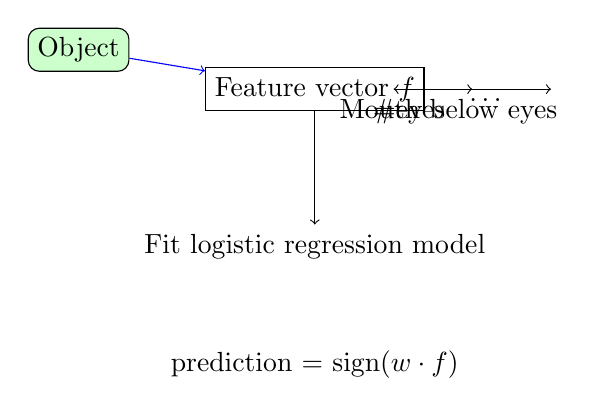
\begin{tikzpicture}
\node[draw, fill=green!20, rounded corners] (object) at (0, 3) {Object};
\node[draw, rectangle, minimum width=2cm, minimum height=0.5cm] (feature_vector) at (3, 2.5) {Feature vector $f$};
\draw[->, blue] (object) -- (feature_vector);
\draw[->] (feature_vector) -- node[below] {\#eyes} (feature_vector -| 4, 1.5);
\draw[->] (feature_vector) -- node[below] {Mouth below eyes} (feature_vector -| 5, 1.5);
\draw[->] (feature_vector) -- node[below] {$\dots$} (feature_vector -| 6, 1.5);
\node[below of=feature_vector, yshift=-1cm] (logistic_regression) {Fit logistic regression model};
\draw[->] (feature_vector) -- (logistic_regression);
\node[below of=logistic_regression, yshift=-0.5cm] (prediction) {prediction = sign($w \cdot f$)};
\end{tikzpicture}
%
\subsection{Description}%
This slide, part of a lecture on Artificial Intelligence Basics, introduces a method for object classification based on invariant features.  The title "Key idea: classify based on invariant features!" is displayed.  A diagram illustrates the process.  An image of an object (likely a portrait) is shown on the left, labeled "Object."  An arrow points from the "Object" to a rectangular box labeled "Feature vector $f$."  This box represents a vector of features extracted from the image.  Below the box, there are arrows pointing down from the box to different feature components.  The features are explicitly listed as "#eyes" and "Mouth below eyes."  There are also ellipses (...), indicating other features that are not explicitly shown.  An arrow points down from the feature vector to the text "Fit logistic regression model."  Finally, the text "prediction = sign($w \cdot f$)" indicates that a logistic regression model is used to calculate a prediction based on the dot product of a weight vector $w$ and the feature vector $f$.  The context suggests that the slide is introducing a method for object recognition that focuses on identifying invariant features, such as the presence of eyes and the position of the mouth, regardless of the object's pose or scale.  The use of logistic regression implies a binary classification task (e.g., is it a face or not?). The diagram uses a `tikzpicture` environment for a more visual representation of the flow of information.%
\subsection{Figures}%
\begin{figure}[H]%
\centering%
\begin{subfigure}[b]{0.15\textwidth}%
\centering%

\includegraphics[width=\textwidth]{/Users/ashoksaravanan/Coding/ScribeLec/server/output/CS 243/lectures/07L2-Vision/figures/22.1.png}%
\caption{}%
\end{subfigure}%
\end{figure}

%
\newpage%
\section{Slide 23}%
\label{sec:Slide23}%
\subsection{Content}%

\textbf{BoF for object categorization}

Need a "visual" dictionary!

G. Cruska et al., "Visual Categorization with Bags of Keypoints", European Conference on Computer Vision, Czech Republic, 2004
%
\subsection{Description}%
This slide, likely part of a lecture on Artificial Intelligence Basics, introduces the Bag-of-Features (BoF) method for object categorization.  The title "BoF for object categorization" clearly states the topic.  Below the title, the slide emphasizes the need for a "visual" dictionary, implying that the method requires a pre-defined collection of visual features to represent objects.  A collage of small images (keypoints?) is displayed, visually representing the concept of a "visual dictionary."  The slide also includes the citation information, attributing the concept to G. Cruska et al. and specifying the publication details: "Visual Categorization with Bags of Keypoints," European Conference on Computer Vision, Czech Republic, 2004.  The context suggests that the slide is part of a discussion on image recognition techniques, specifically how BoF leverages visual features to categorize objects.%
\subsection{Figures}%
\begin{figure}[H]%
\centering%
\begin{subfigure}[b]{0.15\textwidth}%
\centering%

\includegraphics[width=\textwidth]{/Users/ashoksaravanan/Coding/ScribeLec/server/output/CS 243/lectures/07L2-Vision/figures/23.1.png}%
\caption{}%
\end{subfigure}%
\end{figure}

%
\newpage%
\section{Slide 24}%
\label{sec:Slide24}%
\subsection{Content}%
%
\subsection{Description}%
This slide, part of a lecture on Artificial Intelligence Basics, introduces the Bag-of-Features (BoF) method.  The title "BoF: main steps" indicates that the slide details the key steps of the BoF approach.  The text "Characterize objects in terms of parts or local features" describes the core concept of BoF.  The slide likely contains images or diagrams illustrating how objects are broken down into smaller, local features.  The context suggests that the lecture is discussing image recognition techniques, and the BoF method is being presented as a way to represent and categorize objects based on their constituent parts or local features.  The images on the slide (parts of faces, a bicycle, and a violin) visually demonstrate the idea of decomposing an object into its component parts for analysis.%
\subsection{Figures}%
\begin{figure}[H]%
\centering%
\begin{subfigure}[b]{0.15\textwidth}%
\centering%

\includegraphics[width=\textwidth]{/Users/ashoksaravanan/Coding/ScribeLec/server/output/CS 243/lectures/07L2-Vision/figures/24.1.png}%
\caption{}%
\end{subfigure}%
\hspace{0.05\textwidth}%
\begin{subfigure}[b]{0.15\textwidth}%
\centering%

\includegraphics[width=\textwidth]{/Users/ashoksaravanan/Coding/ScribeLec/server/output/CS 243/lectures/07L2-Vision/figures/24.10.png}%
\caption{}%
\end{subfigure}%
\hspace{0.05\textwidth}%
\begin{subfigure}[b]{0.15\textwidth}%
\centering%

\includegraphics[width=\textwidth]{/Users/ashoksaravanan/Coding/ScribeLec/server/output/CS 243/lectures/07L2-Vision/figures/24.11.png}%
\caption{}%
\end{subfigure}%
\hspace{0.05\textwidth}%
\begin{subfigure}[b]{0.15\textwidth}%
\centering%

\includegraphics[width=\textwidth]{/Users/ashoksaravanan/Coding/ScribeLec/server/output/CS 243/lectures/07L2-Vision/figures/24.12.png}%
\caption{}%
\end{subfigure}%
\hspace{0.05\textwidth}%
\begin{subfigure}[b]{0.15\textwidth}%
\centering%

\includegraphics[width=\textwidth]{/Users/ashoksaravanan/Coding/ScribeLec/server/output/CS 243/lectures/07L2-Vision/figures/24.13.png}%
\caption{}%
\end{subfigure}%
\end{figure}

%
\newpage%
\section{Slide 25}%
\label{sec:Slide25}%
\subsection{Content}%

\textbf{BoF: main steps}

Step 1: Features extraction (e.g., Scale-Invariant Feature Transform, SIFT, features)
%
\subsection{Description}%
This slide, part of a lecture on Artificial Intelligence Basics, outlines the main steps of the Bag-of-Features (BoF) method.  The title "BoF: main steps" clearly indicates the topic.  The slide focuses on the first step: "Features extraction."  The text "(e.g., Scale-Invariant Feature Transform, SIFT, features)" provides examples of the types of feature extraction methods used in BoF.  The context suggests that the lecture is discussing image recognition techniques, and the BoF method is being presented as a way to represent and categorize objects based on their constituent features.  A visual representation of an image with marked features (likely keypoints) is present, illustrating the process of extracting features from an image.  The slide likely continues with further steps in the BoF algorithm, as indicated by the "...".%
\subsection{Figures}%
\begin{figure}[H]%
\centering%
\begin{subfigure}[b]{0.15\textwidth}%
\centering%

\includegraphics[width=\textwidth]{/Users/ashoksaravanan/Coding/ScribeLec/server/output/CS 243/lectures/07L2-Vision/figures/25.1.png}%
\caption{}%
\end{subfigure}%
\end{figure}

%
\newpage%
\section{Slide 26}%
\label{sec:Slide26}%
\subsection{Content}%
%
\subsection{Description}%
This slide, part of a lecture on Artificial Intelligence Basics, continues the discussion of the Bag-of-Features (BoF) method.  The title "BoF: main steps (cont'd)" indicates that this is a continuation of a previous slide detailing the steps of the BoF algorithm.  The slide focuses on the second step: "Learn \"visual\" vocabulary."  This step involves extracting features from various images and clustering them to create a "visual vocabulary."  The slide shows a diagram with an arrow pointing down from examples of images (a person, a bicycle, and a violin) to a collection of smaller images, labeled "visual vocabulary."  These smaller images represent the clustered features.  The text "Feature extraction & clustering" describes the process that transforms the initial images into the "visual vocabulary."  The context suggests that the lecture is discussing image recognition techniques, and the BoF method is being presented as a way to represent and categorize objects based on their constituent features.  The slide likely continues with further steps in the BoF algorithm, as indicated by the "(cont'd)" in the title.%
\subsection{Figures}%
\begin{figure}[H]%
\centering%
\begin{subfigure}[b]{0.15\textwidth}%
\centering%

\includegraphics[width=\textwidth]{/Users/ashoksaravanan/Coding/ScribeLec/server/output/CS 243/lectures/07L2-Vision/figures/26.1.png}%
\caption{}%
\end{subfigure}%
\hspace{0.05\textwidth}%
\begin{subfigure}[b]{0.15\textwidth}%
\centering%

\includegraphics[width=\textwidth]{/Users/ashoksaravanan/Coding/ScribeLec/server/output/CS 243/lectures/07L2-Vision/figures/26.10.png}%
\caption{}%
\end{subfigure}%
\hspace{0.05\textwidth}%
\begin{subfigure}[b]{0.15\textwidth}%
\centering%

\includegraphics[width=\textwidth]{/Users/ashoksaravanan/Coding/ScribeLec/server/output/CS 243/lectures/07L2-Vision/figures/26.11.png}%
\caption{}%
\end{subfigure}%
\hspace{0.05\textwidth}%
\begin{subfigure}[b]{0.15\textwidth}%
\centering%

\includegraphics[width=\textwidth]{/Users/ashoksaravanan/Coding/ScribeLec/server/output/CS 243/lectures/07L2-Vision/figures/26.12.png}%
\caption{}%
\end{subfigure}%
\hspace{0.05\textwidth}%
\begin{subfigure}[b]{0.15\textwidth}%
\centering%

\includegraphics[width=\textwidth]{/Users/ashoksaravanan/Coding/ScribeLec/server/output/CS 243/lectures/07L2-Vision/figures/26.13.png}%
\caption{}%
\end{subfigure}%
\end{figure}

%
\newpage%
\section{Slide 27}%
\label{sec:Slide27}%
\subsection{Content}%

\textbf{BoF: main steps (cont'd)}

Step 2: Learn "visual" vocabulary
%
\subsection{Description}%
This slide, part of a lecture on Artificial Intelligence Basics, continues the discussion of the Bag-of-Features (BoF) method.  The title "BoF: main steps (cont'd)" indicates that this is a continuation of a previous slide detailing the steps of the BoF algorithm.  The slide focuses on the second step: "Learn \"visual\" vocabulary."  The slide shows a scatter plot with numerous teal-colored points, which likely represent extracted features from various images.  These points are clustered together, and arrows are drawn from the points to multiple sets of stacked documents, labeled "Features."  The arrows indicate that the features are extracted from the images and then clustered.  A dashed line is drawn through the scatter plot, suggesting a possible clustering boundary.  The context suggests that the lecture is discussing image recognition techniques, and the BoF method is being presented as a way to represent and categorize objects based on their constituent features.  The slide likely continues with further steps in the BoF algorithm, as indicated by the "(cont'd)" in the title.  The visual vocabulary is created by clustering these extracted features.%
\subsection{Figures}%
\begin{figure}[H]%
\centering%
\end{figure}

%
\newpage%
\section{Slide 28}%
\label{sec:Slide28}%
\subsection{Content}%

\textbf{Texture recognition}

Texture is characterized by the repetition of basic elements or textons.

Many times, it is the identity of the textons, not their spatial arrangement, that matters.
%
\subsection{Description}%
This slide, likely part of a lecture on Artificial Intelligence Basics, focuses on texture recognition.  The title, "Texture recognition," clearly indicates the topic.  The text explains that texture is defined by the repetition of basic elements, or "textons."  The key point is that the *identity* of these textons is more important than their spatial arrangement in determining the texture.  The slide likely contains visual examples of textures, which are not included in the provided image.  The examples would illustrate how different textures can be composed of the same textons but arranged differently.  The context of the course suggests that this is part of a discussion on image recognition techniques, specifically how to identify and classify textures based on their constituent elements.%
\subsection{Figures}%
\begin{figure}[H]%
\centering%
\begin{subfigure}[b]{0.15\textwidth}%
\centering%

\includegraphics[width=\textwidth]{/Users/ashoksaravanan/Coding/ScribeLec/server/output/CS 243/lectures/07L2-Vision/figures/28.1.png}%
\caption{}%
\end{subfigure}%
\hspace{0.05\textwidth}%
\begin{subfigure}[b]{0.15\textwidth}%
\centering%

\includegraphics[width=\textwidth]{/Users/ashoksaravanan/Coding/ScribeLec/server/output/CS 243/lectures/07L2-Vision/figures/28.10.png}%
\caption{}%
\end{subfigure}%
\hspace{0.05\textwidth}%
\begin{subfigure}[b]{0.15\textwidth}%
\centering%

\includegraphics[width=\textwidth]{/Users/ashoksaravanan/Coding/ScribeLec/server/output/CS 243/lectures/07L2-Vision/figures/28.11.png}%
\caption{}%
\end{subfigure}%
\hspace{0.05\textwidth}%
\begin{subfigure}[b]{0.15\textwidth}%
\centering%

\includegraphics[width=\textwidth]{/Users/ashoksaravanan/Coding/ScribeLec/server/output/CS 243/lectures/07L2-Vision/figures/28.12.png}%
\caption{}%
\end{subfigure}%
\hspace{0.05\textwidth}%
\begin{subfigure}[b]{0.15\textwidth}%
\centering%

\includegraphics[width=\textwidth]{/Users/ashoksaravanan/Coding/ScribeLec/server/output/CS 243/lectures/07L2-Vision/figures/28.2.png}%
\caption{}%
\end{subfigure}%
\end{figure}

%
\newpage%
\section{Slide 29}%
\label{sec:Slide29}%
\subsection{Content}%
%
\subsection{Description}%
This slide, likely part of a lecture on Artificial Intelligence Basics, focuses on texture recognition.  The title, "Origin 1: Texture recognition," clearly indicates the topic.  The slide displays three examples of textures: a perforated pattern, a grid pattern, and a patterned texture resembling scales.  Each texture is represented by a small grayscale image.  To the right of each texture image, there is a bar graph.  The bars in the graphs represent the frequency of different textons (basic texture elements) found within the corresponding texture image.  The textons are small, simple shapes (squares, circles, etc.) that are visually represented as small icons/symbols within the bar graph.  The orange arrows indicate the process of extracting textons from the texture images and then counting their occurrences.  The context suggests that this is part of a discussion on image recognition techniques, specifically how to identify and classify textures based on their constituent textons and their frequency of occurrence.  The slide is likely illustrating how a texture can be represented by a histogram of its constituent textons, which can then be used for comparison and classification.%
\subsection{Figures}%
\begin{figure}[H]%
\centering%
\begin{subfigure}[b]{0.15\textwidth}%
\centering%

\includegraphics[width=\textwidth]{/Users/ashoksaravanan/Coding/ScribeLec/server/output/CS 243/lectures/07L2-Vision/figures/29.1.png}%
\caption{}%
\end{subfigure}%
\end{figure}

%
\newpage%
\section{Slide 30}%
\label{sec:Slide30}%
\subsection{Content}%

\textbf{BoF Object Categorization (cont'd)}

\textbf{Nearest Neighbor (NN) Classifier}

\textbf{Query image}

\begin{itemize}
    \item Winning class: pink
    \item Assign label of nearest training data point to each test data point
\end{itemize}
%
\subsection{Description}%
This slide, part of a lecture on Artificial Intelligence Basics, details the Nearest Neighbor (NN) classifier within the Bag-of-Features (BoF) object categorization framework.  The title "BoF Object Categorization (cont'd)" indicates this is a continuation of a previous slide.  A small image of a violin is shown on the left, labeled "Query image."  An arrow points from the violin image to a bar graph, also labeled "Query image."  This bar graph likely represents the extracted features (visual vocabulary) from the violin image.  A 3D scatter plot, labeled "Model space," shows various data points in different colors (pink, light blue, orange).  An arrow points from the bar graph to the scatter plot, indicating the mapping of the query image's features to the model space.  The text "Winning class: pink" is below the scatter plot, suggesting that the classifier has determined the query image's class as "pink."  The final bullet point, "Assign label of nearest training data point to each test data point," describes the core principle of the NN classifier.  The context suggests that the lecture is discussing image recognition techniques, and the BoF method is being used to categorize objects based on their visual features.  The slide illustrates how a query image is processed, its features are compared to those of training data, and the label of the nearest training data point is assigned to the query image.%
\subsection{Figures}%
\begin{figure}[H]%
\centering%
\begin{subfigure}[b]{0.15\textwidth}%
\centering%

\includegraphics[width=\textwidth]{/Users/ashoksaravanan/Coding/ScribeLec/server/output/CS 243/lectures/07L2-Vision/figures/30.1.png}%
\caption{}%
\end{subfigure}%
\hspace{0.05\textwidth}%
\begin{subfigure}[b]{0.15\textwidth}%
\centering%

\includegraphics[width=\textwidth]{/Users/ashoksaravanan/Coding/ScribeLec/server/output/CS 243/lectures/07L2-Vision/figures/30.2.png}%
\caption{}%
\end{subfigure}%
\end{figure}

%
\newpage%
\section{Slide 31}%
\label{sec:Slide31}%
\subsection{Content}%
%
\subsection{Description}%
This slide, part of a lecture on Artificial Intelligence Basics, illustrates the Bag-of-Features (BoF) approach to object recognition.  The title clearly states the topic.  A histogram, with pink bars representing frequencies, shows the distribution of "codewords" extracted from an image.  The x-axis likely represents different codewords (visual vocabulary), and the y-axis represents the frequency of each codeword.  A grayscale image of a car is shown in the upper right corner, with bounding boxes (red and green squares) highlighting detected objects.  These boxes correspond to the codewords in the histogram.  The codewords are small grayscale images (visual vocabulary) displayed below the histogram.  The green and red boxes in the image correspond to the codewords with the highest frequency in the histogram.  The context suggests that the slide is explaining how the BoF method extracts visual features (codewords) from an image, counts their occurrences, and uses this frequency distribution to represent the image for object recognition.  The bounding boxes in the image indicate that the method is capable of detecting and localizing objects within the image.%
\subsection{Figures}%
\begin{figure}[H]%
\centering%
\begin{subfigure}[b]{0.15\textwidth}%
\centering%

\includegraphics[width=\textwidth]{/Users/ashoksaravanan/Coding/ScribeLec/server/output/CS 243/lectures/07L2-Vision/figures/31.1.png}%
\caption{}%
\end{subfigure}%
\end{figure}

%
\newpage%
\section{Slide 32}%
\label{sec:Slide32}%
\subsection{Content}%
%
\subsection{Description}%
This slide, part of a lecture on Artificial Intelligence Basics, discusses the Bag-of-Features (BoF) approach to object recognition.  The title clearly states the topic.  The slide shows a series of bar graphs labeled "category models" and "Class 1," "...," "Class N."  These graphs likely represent the frequency distribution of visual features (codewords or visual vocabulary) extracted from images belonging to different object categories.  The x-axis of each bar graph likely represents different codewords, and the y-axis represents the frequency of each codeword.  A 3D scatter plot, labeled "Model space," is shown on the right side of the slide.  The scatter plot displays data points in different colors (e.g., cyan and pink), likely representing the category models for different classes.  Arrows are not explicitly shown, but the arrangement suggests a mapping from the category models (bar graphs) to the model space (scatter plot).  The context suggests that the BoF method extracts visual features from images, counts their occurrences, and uses this frequency distribution to represent the image for object recognition.  The bar graphs and scatter plot illustrate how the BoF method creates a representation of an image's visual content and how these representations can be used to classify objects.%
\subsection{Figures}%
\begin{figure}[H]%
\centering%
\begin{subfigure}[b]{0.15\textwidth}%
\centering%

\includegraphics[width=\textwidth]{/Users/ashoksaravanan/Coding/ScribeLec/server/output/CS 243/lectures/07L2-Vision/figures/32.1.png}%
\caption{}%
\end{subfigure}%
\end{figure}

%
\newpage%
\section{Slide 33}%
\label{sec:Slide33}%
\subsection{Content}%

\textbf{Noise}
%
\subsection{Description}%
This slide, likely part of a presentation on a topic related to signal processing or image analysis, simply displays the word "Noise".  There are no other elements on the slide, suggesting that this is a title slide or a placeholder for a section discussing noise in the context of the course, Artificial Intelligence Basics.  The context of the course is crucial for understanding the specific type of noise being discussed (e.g., Gaussian noise, salt-and-pepper noise, etc.).%
\subsection{Figures}%
\begin{figure}[H]%
\centering%
\end{figure}

%
\newpage%
\section{Slide 34}%
\label{sec:Slide34}%
\subsection{Content}%
%
\subsection{Description}%

This slide, part of a lecture on Artificial Intelligence Basics, explains how images are represented in MATLAB.  It states that color images are represented as matrices with multiple channels (e.g., RGB).  A grayscale image would have only one channel.  The slide introduces the notation "im" to represent an image.  The key points are:

* **im(1, 1, 1):** This represents the top-left pixel value in the red (R) channel of the image.  The first two indices (1, 1) specify the row and column position, and the third index (1) specifies the channel.

* **im(y, x, b):** This represents the pixel at row y, column x, and channel b.  This notation shows how to access any pixel in the image, specifying the row, column, and channel.

* **im(N, M, 3):** This represents the bottom-right pixel in the blue (B) channel.  N and M are the total number of rows and columns in the image, respectively.  The 3 indicates the third channel, which is blue in the RGB color model.

The slide also includes a table (not in LaTeX format) showing numerical values for each pixel in the R, G, and B channels.  This table visually demonstrates how the image data is stored in a matrix format.  The table is adapted from Derek Hoiem, indicating a potential source for the information.  The context of the course is crucial for understanding the importance of image representation in computer vision tasks, such as object recognition and image processing.
%
\subsection{Figures}%
\begin{figure}[H]%
\centering%
\end{figure}

%
\newpage%
\section{Slide 35}%
\label{sec:Slide35}%
\subsection{Content}%
%
\subsection{Description}%
This slide, part of a lecture on Artificial Intelligence Basics, introduces the concept of noise in image analysis.  The title "Enter: Noise" indicates the topic of discussion.  The text explains that even identical objects or scenes captured in multiple images will appear different due to noise.  The slide shows a series of grayscale images, likely of the same scene, but with variations.  These variations represent the noise present in the images.  The question "How could we reduce the noise?" is posed, suggesting that the lecture will discuss methods for mitigating noise in image data.  The name "Kristen Grauman" is present at the bottom, likely indicating the presenter or author of the slide.  The context of the course is crucial for understanding the specific types of noise being discussed (e.g., Gaussian noise, salt-and-pepper noise, etc.) and the methods for noise reduction that might be covered in subsequent slides.  The images on the slide visually illustrate the variability introduced by noise in image acquisition.%
\subsection{Figures}%
\begin{figure}[H]%
\centering%
\begin{subfigure}[b]{0.15\textwidth}%
\centering%

\includegraphics[width=\textwidth]{/Users/ashoksaravanan/Coding/ScribeLec/server/output/CS 243/lectures/07L2-Vision/figures/35.1.png}%
\caption{}%
\end{subfigure}%
\hspace{0.05\textwidth}%
\begin{subfigure}[b]{0.15\textwidth}%
\centering%

\includegraphics[width=\textwidth]{/Users/ashoksaravanan/Coding/ScribeLec/server/output/CS 243/lectures/07L2-Vision/figures/35.2.png}%
\caption{}%
\end{subfigure}%
\hspace{0.05\textwidth}%
\begin{subfigure}[b]{0.15\textwidth}%
\centering%

\includegraphics[width=\textwidth]{/Users/ashoksaravanan/Coding/ScribeLec/server/output/CS 243/lectures/07L2-Vision/figures/35.3.png}%
\caption{}%
\end{subfigure}%
\hspace{0.05\textwidth}%
\begin{subfigure}[b]{0.15\textwidth}%
\centering%

\includegraphics[width=\textwidth]{/Users/ashoksaravanan/Coding/ScribeLec/server/output/CS 243/lectures/07L2-Vision/figures/35.4.png}%
\caption{}%
\end{subfigure}%
\hspace{0.05\textwidth}%
\begin{subfigure}[b]{0.15\textwidth}%
\centering%

\includegraphics[width=\textwidth]{/Users/ashoksaravanan/Coding/ScribeLec/server/output/CS 243/lectures/07L2-Vision/figures/35.5.png}%
\caption{}%
\end{subfigure}%
\end{figure}

%
\newpage%
\section{Slide 36}%
\label{sec:Slide36}%
\subsection{Content}%

\textbf{Common types of noise}

Salt and pepper noise: random occurrences of black and white pixels \\
Impulse noise: random occurrences of white pixels \\
Gaussian noise: variations in intensity drawn from a Gaussian normal distribution
%
\subsection{Description}%
This slide, likely part of a presentation on image processing or computer vision within the context of Artificial Intelligence Basics, details different types of noise commonly encountered in image data.  It lists three primary types:

* **Salt and pepper noise:** Characterized by random occurrences of black and white pixels within the image.  This type of noise creates a "salt-and-pepper" effect, with random dark and light spots.  Visual examples of this type of noise are shown on the slide.

* **Impulse noise:**  Similar to salt-and-pepper noise, but specifically characterized by random occurrences of white pixels.  The visual effect is similar, but the presence of white pixels is more prominent.  Again, visual examples are shown.

* **Gaussian noise:**  This type of noise introduces variations in the intensity of pixels, drawn from a Gaussian (normal) distribution.  This results in a more subtle form of noise, appearing as a blurring or grainy effect.  The visual examples on the slide illustrate the effect of Gaussian noise.

The slide also includes images illustrating each type of noise, showing the original image and the image corrupted by the respective noise type.  The source of the information is credited to "S. Seitz."  The context of the course is crucial for understanding the importance of noise reduction techniques in image processing tasks, such as those used in computer vision applications within AI.%
\subsection{Figures}%
\begin{figure}[H]%
\centering%
\begin{subfigure}[b]{0.15\textwidth}%
\centering%

\includegraphics[width=\textwidth]{/Users/ashoksaravanan/Coding/ScribeLec/server/output/CS 243/lectures/07L2-Vision/figures/36.1.png}%
\caption{}%
\end{subfigure}%
\end{figure}

%
\newpage%
\section{Slide 37}%
\label{sec:Slide37}%
\subsection{Content}%

\textbf{Gaussian noise}

Ideal Image \quad Noise process \\
$f(x, y) = f(x, y) + \eta(x, y)$ \\
Gaussian i.i.d. ("white") noise: \\
$\eta(x, y) \sim \mathcal{N}(\mu, \sigma^2)$ \\
>> noise = randn(size(im)).*sigma; \\
>> output = im + noise; \\
What is impact of the sigma? \\
Fig: M. Hebert
%
\subsection{Description}%
This slide discusses Gaussian noise in image processing, a common type of noise encountered in image acquisition.  The slide shows a grayscale image, likely representing an ideal image, and a second image that has been corrupted by Gaussian noise.  The text describes the process of adding Gaussian noise to an image.  The equation $f(x, y) = f(x, y) + \eta(x, y)$ represents the process, where $f(x, y)$ is the ideal image, $\eta(x, y)$ is the Gaussian noise, and the result is the noisy image.  The notation $\eta(x, y) \sim \mathcal{N}(\mu, \sigma^2)$ indicates that the noise is modeled by a Gaussian distribution with mean $\mu$ and variance $\sigma^2$.  The MATLAB code snippets `noise = randn(size(im)).*sigma;` and `output = im + noise;` illustrate how Gaussian noise is added to an image in MATLAB.  The question "What is the impact of the sigma?" suggests that the lecture will discuss how the variance parameter $\sigma^2$ affects the appearance of the noisy image.  The context of the course (Artificial Intelligence Basics, likely a module on image processing) is crucial for understanding the importance of noise reduction techniques in computer vision applications.  The figure is attributed to M. Hebert.%
\subsection{Figures}%
\begin{figure}[H]%
\centering%
\begin{subfigure}[b]{0.15\textwidth}%
\centering%

\includegraphics[width=\textwidth]{/Users/ashoksaravanan/Coding/ScribeLec/server/output/CS 243/lectures/07L2-Vision/figures/37.1.png}%
\caption{}%
\end{subfigure}%
\end{figure}

%
\newpage%
\section{Slide 38}%
\label{sec:Slide38}%
\subsection{Content}%

\textbf{First attempt at a solution} \\
Let's replace each pixel with an average of all the values in its neighborhood \\
\textbf{Assumptions}: \\
\begin{itemize}
    \item Expect pixels to be like their neighbors
    \item Expect noise processes to be independent from pixel to pixel
\end{itemize}
%
\subsection{Description}%
This slide, likely part of a lecture on image processing within the context of Artificial Intelligence Basics, outlines a first approach to noise reduction in images.  The title "First attempt at a solution" indicates that this is a proposed method, and the text describes the method as replacing each pixel with the average of all the values in its neighborhood.  The assumptions listed below the method describe the conditions under which this approach might be effective.  The first assumption, "Expect pixels to be like their neighbors," implies that the method assumes spatial correlation in the image data, meaning that neighboring pixels tend to have similar values.  The second assumption, "Expect noise processes to be independent from pixel to pixel," implies that the noise affecting each pixel is not correlated with the noise affecting its neighbors.  The name "Kristen Grauman" at the bottom suggests the presenter or author of the slide.  The context of the course is crucial for understanding the specific types of noise being considered and the potential limitations of this averaging approach.%
\subsection{Figures}%
\begin{figure}[H]%
\centering%
\end{figure}

%
\newpage%
\section{Slide 39}%
\label{sec:Slide39}%
\subsection{Content}%
%
\subsection{Description}%
This slide, part of a lecture on image processing within the context of Artificial Intelligence Basics, introduces a basic noise reduction technique.  The title "First attempt at a solution" indicates that this is a proposed method for reducing noise in images.  The text describes the method as replacing each pixel with the average of all the values in its neighborhood.  The "Moving average in 1D" section likely refers to a graphical illustration of how this method works in a one-dimensional context.  Two graphs are shown, one representing the original data (likely an image intensity profile) with significant fluctuations, and the other representing the data after applying a moving average filter.  The second graph shows a smoothed version of the original data, with the fluctuations reduced.  The visual representation demonstrates how the moving average filter averages the values in a neighborhood of pixels to reduce noise.  The source is credited to "S. Marschner."  The context of the course suggests that this slide is part of a discussion on image processing techniques for noise reduction, which are crucial for various computer vision tasks in AI.%
\subsection{Figures}%
\begin{figure}[H]%
\centering%
\begin{subfigure}[b]{0.15\textwidth}%
\centering%

\includegraphics[width=\textwidth]{/Users/ashoksaravanan/Coding/ScribeLec/server/output/CS 243/lectures/07L2-Vision/figures/39.1.png}%
\caption{}%
\end{subfigure}%
\hspace{0.05\textwidth}%
\begin{subfigure}[b]{0.15\textwidth}%
\centering%

\includegraphics[width=\textwidth]{/Users/ashoksaravanan/Coding/ScribeLec/server/output/CS 243/lectures/07L2-Vision/figures/39.2.png}%
\caption{}%
\end{subfigure}%
\hspace{0.05\textwidth}%
\begin{subfigure}[b]{0.15\textwidth}%
\centering%

\includegraphics[width=\textwidth]{/Users/ashoksaravanan/Coding/ScribeLec/server/output/CS 243/lectures/07L2-Vision/figures/39.3.png}%
\caption{}%
\end{subfigure}%
\hspace{0.05\textwidth}%
\begin{subfigure}[b]{0.15\textwidth}%
\centering%

\includegraphics[width=\textwidth]{/Users/ashoksaravanan/Coding/ScribeLec/server/output/CS 243/lectures/07L2-Vision/figures/39.4.png}%
\caption{}%
\end{subfigure}%
\hspace{0.05\textwidth}%
\begin{subfigure}[b]{0.15\textwidth}%
\centering%

\includegraphics[width=\textwidth]{/Users/ashoksaravanan/Coding/ScribeLec/server/output/CS 243/lectures/07L2-Vision/figures/39.5.png}%
\caption{}%
\end{subfigure}%
\end{figure}

%
\newpage%
\section{Slide 40}%
\label{sec:Slide40}%
\subsection{Content}%

\textbf{Weighted Moving Average} \\
Can add weights to our moving average \\
Weights \\
[1, 1, 1, 1, 1]/5
%
\subsection{Description}%
This slide, part of a lecture on image processing within the context of Artificial Intelligence Basics, introduces the concept of a weighted moving average.  The title "Weighted Moving Average" indicates that this is a method for smoothing data, similar to a simple moving average, but with different weights assigned to the data points within the neighborhood.  The text "Can add weights to our moving average" explains the key difference from a simple moving average.  The line "Weights [1, 1, 1, 1, 1]/5" shows an example of weights assigned to a neighborhood of 5 data points.  Each data point in the neighborhood is given a weight of 1, and the sum of these weights is divided by 5 to normalize the weights.  This implies that each data point in the neighborhood contributes equally to the average.  A graph is included, showing a noisy signal (represented by discrete data points) and a smoothed version of the signal (likely the result of applying a weighted moving average).  The graph visually demonstrates the effect of the weighted moving average on the data.  The source is credited to "S. Marschner."  The context of the course suggests that this slide is part of a discussion on image processing techniques for noise reduction, which are crucial for various computer vision tasks in AI.%
\subsection{Figures}%
\begin{figure}[H]%
\centering%
\begin{subfigure}[b]{0.15\textwidth}%
\centering%

\includegraphics[width=\textwidth]{/Users/ashoksaravanan/Coding/ScribeLec/server/output/CS 243/lectures/07L2-Vision/figures/40.1.png}%
\caption{}%
\end{subfigure}%
\end{figure}

%
\newpage%
\section{Slide 41}%
\label{sec:Slide41}%
\subsection{Content}%

\textbf{Weighted Moving Average} \\
Non-uniform weights \\
$[1, 4, 6, 4, 1]/16$ \\
Central pixel = $10 \cdot 1 + 14 \cdot 4 + 12 \cdot 6 + 13 \cdot 4 + 20 \cdot 1$
%
\subsection{Description}%
This slide discusses a weighted moving average technique for image processing, likely within the context of Artificial Intelligence Basics.  The title "Weighted Moving Average" indicates the focus on a method that assigns different weights to neighboring pixels when calculating the average value of a central pixel.  "Non-uniform weights [1, 4, 6, 4, 1]/16" shows the specific weights assigned to the pixels in a neighborhood.  The weights are not all equal, implying that pixels closer to the central pixel have a greater influence on the average.  The formula "Central pixel = $10 \cdot 1 + 14 \cdot 4 + 12 \cdot 6 + 13 \cdot 4 + 20 \cdot 1$" demonstrates how the weighted average is calculated.  The numbers (10, 14, 12, 13, 20) likely represent the pixel values in the neighborhood, and the corresponding weights (1, 4, 6, 4, 1) are used to calculate the weighted sum.  A graph is included, showing a noisy signal (represented by discrete data points) and a smoothed version of the signal (likely the result of applying a weighted moving average).  The graph visually demonstrates the effect of the weighted moving average on the data.  The values 10, 14, 12, 13, and 20 are the pixel values, and the weights are used to calculate the weighted average of the central pixel. The notation "/16" indicates that the weights are normalized by dividing by 16.  The source is credited to "S. Marschner."  The context of the course suggests that this slide is part of a discussion on image processing techniques for noise reduction, which are crucial for various computer vision tasks in AI.%
\subsection{Figures}%
\begin{figure}[H]%
\centering%
\begin{subfigure}[b]{0.15\textwidth}%
\centering%

\includegraphics[width=\textwidth]{/Users/ashoksaravanan/Coding/ScribeLec/server/output/CS 243/lectures/07L2-Vision/figures/41.1.png}%
\caption{}%
\end{subfigure}%
\hspace{0.05\textwidth}%
\begin{subfigure}[b]{0.15\textwidth}%
\centering%

\includegraphics[width=\textwidth]{/Users/ashoksaravanan/Coding/ScribeLec/server/output/CS 243/lectures/07L2-Vision/figures/41.2.png}%
\caption{}%
\end{subfigure}%
\end{figure}

%
\newpage%
\section{Slide 42}%
\label{sec:Slide42}%
\subsection{Content}%
%
\subsection{Description}%
This slide, part of a lecture on image processing within the context of Artificial Intelligence Basics, demonstrates a moving average filter in a 2D context.  The title "Moving Average In 2D" indicates the focus on a technique for smoothing image data.  The slide shows two matrices, $F[x, y]$ and $G[x, y]$.  $F[x, y]$ represents an input image (or a section of an image) where values are likely pixel intensities (e.g., 90).  The matrix $F[x, y]$ has a block of 90s in the middle, surrounded by zeros.  The matrix $G[x, y]$ is an output matrix, which will be the result of applying the moving average filter to $F[x, y]$.  The top-left corner of $F[x, y]$ has a 3x3 block of zeros, which is likely the neighborhood being considered for the moving average calculation.  The $G[x, y]$ matrix shows a single cell with a value of 0.  The notation suggests that the moving average is being applied to a specific pixel location (x, y) in the image.  The 3x3 block of 1s in the top left corner of $F[x, y]$ likely represents the filter kernel used for the moving average calculation.  The values in the $F[x, y]$ matrix are likely pixel intensities, and the moving average filter is used to reduce noise in the image.  The source is credited to "S. Seitz."  The context of the course suggests that this slide is part of a discussion on image processing techniques for noise reduction, which are crucial for various computer vision tasks in AI.%
\subsection{Figures}%
\begin{figure}[H]%
\centering%
\end{figure}

%
\newpage%
\section{Slide 43}%
\label{sec:Slide43}%
\subsection{Content}%
%
\subsection{Description}%
This slide, part of a lecture on image processing within the context of Artificial Intelligence Basics, demonstrates a 2D moving average filter.  The title "Moving Average In 2D" indicates the focus on a technique for smoothing image data.  The slide shows two matrices, $F[x, y]$ and $G[x, y]$.  $F[x, y]$ represents an input image (or a section of an image) where values are likely pixel intensities.  The matrix $F[x, y]$ has a central 3x3 block of the value 90, surrounded by zeros.  The matrix $G[x, y]$ is the output matrix, which will be the result of applying the moving average filter to $F[x, y]$.  The top-left corner of $G[x, y]$ has a single cell with the value 10.  This indicates that the moving average filter has been applied to the corresponding pixel location (x, y) in the input image $F[x, y]$.  The 3x3 block of 90s in $F[x, y]$ likely represents the neighborhood being considered for the moving average calculation.  The value 10 in $G[x, y]$ is the result of averaging the values within the 3x3 neighborhood in $F[x, y]$.  The values in the $F[x, y]$ matrix are likely pixel intensities, and the moving average filter is used to reduce noise in the image.  The notation suggests that the moving average is being applied to a specific pixel location (x, y) in the image. The context of the course suggests that this slide is part of a discussion on image processing techniques for noise reduction, which are crucial for various computer vision tasks in AI.%
\subsection{Figures}%
\begin{figure}[H]%
\centering%
\end{figure}

%
\newpage%
\section{Slide 44}%
\label{sec:Slide44}%
\subsection{Content}%
%
\subsection{Description}%
This slide, part of a lecture on image processing within the context of Artificial Intelligence Basics, demonstrates a 2D moving average filter.  The title "Moving Average In 2D" indicates the focus on a technique for smoothing image data.  The slide shows two matrices, $F[x, y]$ and $G[x, y]$.  $F[x, y]$ represents an input image (or a section of an image) where values are likely pixel intensities.  The matrix $F[x, y]$ has a central 3x3 block of the value 90, surrounded by zeros.  The matrix $G[x, y]$ is the output matrix, which will be the result of applying the moving average filter to $F[x, y]$.  The top-left corner of $G[x, y]$ has a single cell with the value 10, and the cell immediately to the right has the value 20. This indicates that the moving average filter has been applied to the corresponding pixel location (x, y) in the input image $F[x, y]$. The 3x3 block of 90s in $F[x, y]$ likely represents the neighborhood being considered for the moving average calculation. The values 10 and 20 in $G[x, y]$ are the result of averaging the values within the 3x3 neighborhood in $F[x, y]$. The values in the $F[x, y]$ matrix are likely pixel intensities, and the moving average filter is used to reduce noise in the image. The notation suggests that the moving average is being applied to a specific pixel location (x, y) in the image. The context of the course suggests that this slide is part of a discussion on image processing techniques for noise reduction, which are crucial for various computer vision tasks in AI.  The source is credited to "S. Seitz."  The presence of the matrix notation and the values 90 and 0 suggest that this is a demonstration of a simple moving average filter, where the average of the values in a 3x3 neighborhood is calculated and placed in the corresponding output matrix position.%
\subsection{Figures}%
\begin{figure}[H]%
\centering%
\end{figure}

%
\newpage%
\section{Slide 45}%
\label{sec:Slide45}%
\subsection{Content}%
%
\subsection{Description}%
This slide, part of a lecture on image processing within the context of Artificial Intelligence Basics, demonstrates a 2D moving average filter.  The title "Moving Average In 2D" indicates the focus on a technique for smoothing image data.  The slide displays two matrices, $F[x, y]$ and $G[x, y]$.  $F[x, y]$ represents an input image (or a section of an image) where values are likely pixel intensities.  The matrix $F[x, y]$ shows a 7x7 block of mostly zeros, with a central 3x3 block containing the value 90.  The matrix $G[x, y]$ is the output matrix, which will be the result of applying the moving average filter to $F[x, y]$.  The top-left corner of $G[x, y]$ has a single cell with the value 0, followed by 10, 20, and 30.  This indicates that the moving average filter has been applied to the corresponding pixel location (x, y) in the input image $F[x, y]$. The 3x3 block of 90s in $F[x, y]$ likely represents the neighborhood being considered for the moving average calculation. The values 0, 10, 20, and 30 in $G[x, y]$ are the result of averaging the values within the 3x3 neighborhood in $F[x, y]$. The values in the $F[x, y]$ matrix are likely pixel intensities, and the moving average filter is used to reduce noise in the image. The notation suggests that the moving average is being applied to a specific pixel location (x, y) in the image. The context of the course suggests that this slide is part of a discussion on image processing techniques for noise reduction, which are crucial for various computer vision tasks in AI. The source is credited to "S. Seitz."  The presence of the matrices and the values 90 and 0 suggest that this is a demonstration of a simple moving average filter, where the average of the values in a 3x3 neighborhood is calculated and placed in the corresponding output matrix position. The example shows the result of applying the filter to a specific pixel location in the image.%
\subsection{Figures}%
\begin{figure}[H]%
\centering%
\end{figure}

%
\newpage%
\section{Slide 46}%
\label{sec:Slide46}%
\subsection{Content}%
%
\subsection{Description}%
This slide, part of a lecture on image processing within the context of Artificial Intelligence Basics, demonstrates a 2D moving average filter.  The title "Moving Average In 2D" indicates the focus on a technique for smoothing image data.  The slide shows two matrices, $F[x, y]$ and $G[x, y]$.  $F[x, y]$ represents an input image (or a section of an image) where values are likely pixel intensities.  The matrix $F[x, y]$ is a 7x7 matrix with a central 3x3 block containing the value 90, surrounded by zeros.  The matrix $G[x, y]$ is the output matrix, which will be the result of applying the moving average filter to $F[x, y]$.  The top-left corner of $G[x, y]$ has a value of 0, followed by 10, 20, and 30. This indicates that the moving average filter has been applied to the corresponding pixel location (x, y) in the input image $F[x, y]$. The 3x3 block of 90s in $F[x, y]$ represents the neighborhood being considered for the moving average calculation. The values in $G[x, y]$ are the result of averaging the values within the 3x3 neighborhood in $F[x, y]$. The values in the $F[x, y]$ matrix are likely pixel intensities, and the moving average filter is used to reduce noise in the image. The notation suggests that the moving average is being applied to a specific pixel location (x, y) in the image. The context of the course suggests that this slide is part of a discussion on image processing techniques for noise reduction, which are crucial for various computer vision tasks in AI. The source is credited to "S. Seitz."  The example shows the result of applying the filter to a specific pixel location in the image, where the average of the 3x3 neighborhood centered on that pixel is calculated and placed in the corresponding output matrix position.%
\subsection{Figures}%
\begin{figure}[H]%
\centering%
\end{figure}

%
\newpage%
\section{Slide 47}%
\label{sec:Slide47}%
\subsection{Content}%
%
\subsection{Description}%
This slide from a lecture on Artificial Intelligence Basics, specifically focusing on image processing, demonstrates a 2D moving average filter.  The matrix $F[x, y]$ represents an input image (or a section of an image) where values are likely pixel intensities.  The matrix $F[x, y]$ is a 7x7 matrix with a central 3x3 block containing the value 90, surrounded by zeros.  The matrix $G[x, y]$ is the output matrix, which is the result of applying the moving average filter to $F[x, y]$.  The values in $G[x, y]$ are the result of averaging the values within a 3x3 neighborhood in $F[x, y]$.  For example, the top-left value in $G[x, y]$ (0) is likely the average of the 3x3 neighborhood centered on the corresponding pixel in $F[x, y]$.  The values in $G[x, y]$ are calculated by averaging the corresponding 3x3 neighborhood in $F[x, y]$.  The example shows the result of applying the filter to a specific pixel location in the image.  The context of the course suggests that this slide is part of a discussion on image processing techniques for noise reduction, which are crucial for various computer vision tasks in AI. The source is credited to "S. Seitz."  The grayscale shading in the $G[x, y]$ matrix likely represents the intensity values, with darker shades corresponding to lower average values and lighter shades to higher average values.%
\subsection{Figures}%
\begin{figure}[H]%
\centering%
\end{figure}

%
\newpage%
\section{Slide 48}%
\label{sec:Slide48}%
\subsection{Content}%
%
\subsection{Description}%
This slide, part of a lecture on Artificial Intelligence Basics, specifically image processing, displays an example of noise reduction using a mean filter.  Two grayscale images of a cat's head are shown side-by-side. The image on the left appears to have significant noise, characterized by speckled, uneven shading. The image on the right, which is the result of applying a mean filter, shows a smoother, less noisy representation of the cat's head.  The title "Noise reduction using mean filtering" clearly indicates the topic of the slide.  The images demonstrate the effect of the mean filter in reducing the random variations in pixel intensities, effectively smoothing out the image and removing noise.  The context of the course suggests that this slide is part of a discussion on image processing techniques for noise reduction, which are crucial for various computer vision tasks in AI.  The example visually illustrates the application of a mean filter to reduce noise in an image.
%
\subsection{Figures}%
\begin{figure}[H]%
\centering%
\begin{subfigure}[b]{0.15\textwidth}%
\centering%

\includegraphics[width=\textwidth]{/Users/ashoksaravanan/Coding/ScribeLec/server/output/CS 243/lectures/07L2-Vision/figures/48.1.png}%
\caption{}%
\end{subfigure}%
\hspace{0.05\textwidth}%
\begin{subfigure}[b]{0.15\textwidth}%
\centering%

\includegraphics[width=\textwidth]{/Users/ashoksaravanan/Coding/ScribeLec/server/output/CS 243/lectures/07L2-Vision/figures/48.2.png}%
\caption{}%
\end{subfigure}%
\end{figure}

%
\newpage%
\section{Slide 49}%
\label{sec:Slide49}%
\subsection{Content}%
%
\subsection{Description}%
This slide, part of a lecture on Artificial Intelligence Basics, specifically image processing, introduces the concept of image filtering.  It defines image filtering as computing a function of the local neighborhood at each pixel in an image.  The process involves a "filter" or mask that dictates how to combine values from neighboring pixels.  The filter is applied element-wise to the image patch.  The slide then lists common uses of image filtering, including enhancing images (e.g., denoising, resizing), extracting image information (e.g., texture, edges), and detecting patterns (e.g., template matching).  The source is credited to Derek Hoiem.  The context of the course suggests that this slide is part of a larger discussion on image processing techniques, which are crucial for various computer vision tasks in AI.%
\subsection{Figures}%
\begin{figure}[H]%
\centering%
\end{figure}

%
\newpage%
\section{Slide 50}%
\label{sec:Slide50}%
\subsection{Content}%
%
\subsection{Description}%
This slide from a lecture on Artificial Intelligence Basics, focusing on image processing, demonstrates a blurring operation using a mean filter.  The image on the left, labeled "Original (f)," shows a grayscale image, likely a portion of a face. The image on the right, labeled "Blur (with a mean filter) (g)," shows the same image after applying a 3x3 mean filter. The middle section displays the kernel (k) used for the filtering operation. The kernel is a 3x3 matrix with all elements equal to 1, and the entire matrix is divided by 9. This indicates that the filter calculates the average of the 9 pixels within a 3x3 neighborhood centered on each pixel in the original image to produce the blurred image.  The process effectively reduces high-frequency components in the image, smoothing out details and reducing noise. The source is credited to D. Lowe. The context of the course suggests that this slide is part of a discussion on image processing techniques, which are crucial for various computer vision tasks in AI.%
\subsection{Figures}%
\begin{figure}[H]%
\centering%
\begin{subfigure}[b]{0.15\textwidth}%
\centering%

\includegraphics[width=\textwidth]{/Users/ashoksaravanan/Coding/ScribeLec/server/output/CS 243/lectures/07L2-Vision/figures/50.1.png}%
\caption{}%
\end{subfigure}%
\hspace{0.05\textwidth}%
\begin{subfigure}[b]{0.15\textwidth}%
\centering%

\includegraphics[width=\textwidth]{/Users/ashoksaravanan/Coding/ScribeLec/server/output/CS 243/lectures/07L2-Vision/figures/50.2.png}%
\caption{}%
\end{subfigure}%
\hspace{0.05\textwidth}%
\begin{subfigure}[b]{0.15\textwidth}%
\centering%

\includegraphics[width=\textwidth]{/Users/ashoksaravanan/Coding/ScribeLec/server/output/CS 243/lectures/07L2-Vision/figures/50.3.png}%
\caption{}%
\end{subfigure}%
\end{figure}

%
\newpage%
\section{Slide 51}%
\label{sec:Slide51}%
\subsection{Content}%
%
\subsection{Description}%
This slide, part of a lecture on Artificial Intelligence Basics, specifically image processing, demonstrates the identity filter.  It shows a grayscale image (likely a portion of a face) labeled "Original (f)".  A 3x3 kernel (k) is presented, containing the values:
```
0 0 0
0 1 0
0 0 0
```
The asterisk (*) symbol indicates the convolution operation.  The result of applying this filter to the original image is an "Identical image (g)," visually identical to the original image.  This demonstrates that the identity filter does not alter the image; it simply passes the original pixel values through the filter.  The source is credited to D. Lowe. The context of the course suggests that this slide is part of a discussion on image processing techniques, which are crucial for various computer vision tasks in AI.  The example visually illustrates the concept of an identity filter, which is a fundamental building block for more complex image processing operations.%
\subsection{Figures}%
\begin{figure}[H]%
\centering%
\begin{subfigure}[b]{0.15\textwidth}%
\centering%

\includegraphics[width=\textwidth]{/Users/ashoksaravanan/Coding/ScribeLec/server/output/CS 243/lectures/07L2-Vision/figures/51.1.png}%
\caption{}%
\end{subfigure}%
\hspace{0.05\textwidth}%
\begin{subfigure}[b]{0.15\textwidth}%
\centering%

\includegraphics[width=\textwidth]{/Users/ashoksaravanan/Coding/ScribeLec/server/output/CS 243/lectures/07L2-Vision/figures/51.2.png}%
\caption{}%
\end{subfigure}%
\end{figure}

%
\newpage%
\section{Slide 52}%
\label{sec:Slide52}%
\subsection{Content}%
%
\subsection{Description}%
This slide, part of a lecture on Artificial Intelligence Basics, specifically image processing, demonstrates the effect of sharpening an image.  Two images are presented side-by-side. The image on the left is labeled "Before" and shows a grayscale image, likely a portrait of Albert Einstein. The image on the right, labeled "After," displays the same image after a sharpening filter has been applied.  The sharpening operation has enhanced the details and edges in the image, making them more distinct.  The difference is visually apparent in the image, with sharper lines and greater contrast. The source is credited to D. Lowe. The context of the course suggests that this slide is part of a discussion on image processing techniques, which are crucial for various computer vision tasks in AI, specifically highlighting the effect of sharpening filters on image quality.%
\subsection{Figures}%
\begin{figure}[H]%
\centering%
\begin{subfigure}[b]{0.15\textwidth}%
\centering%

\includegraphics[width=\textwidth]{/Users/ashoksaravanan/Coding/ScribeLec/server/output/CS 243/lectures/07L2-Vision/figures/52.1.png}%
\caption{}%
\end{subfigure}%
\end{figure}

%
\newpage%
\section{Slide 53}%
\label{sec:Slide53}%
\subsection{Content}%
%
\subsection{Description}%
This slide, part of a lecture on Artificial Intelligence Basics, specifically image processing, demonstrates the concept of image sharpening.  It visually shows how sharpening works by reversing the effect of blurring.  The top row shows an original image (f) and a blurred version (g).  The middle row shows the original image (f) with the blurred image (g) added back to it. The bottom row shows the original image (f) with a scaled version of the blurred image (g) added to it, represented by the term + α.  The text "Sharpening" and "What does blurring take away?" above the images suggest that the slide is explaining how to reverse the blurring effect to sharpen an image. The images are grayscale portraits of Albert Einstein. The context of the course suggests that this slide is part of a discussion on image processing techniques, which are crucial for various computer vision tasks in AI, specifically highlighting the process of sharpening images by reversing the blurring operation. The use of the term "α" (alpha) implies a scaling factor applied to the blurred image before adding it to the original.%
\subsection{Figures}%
\begin{figure}[H]%
\centering%
\begin{subfigure}[b]{0.15\textwidth}%
\centering%

\includegraphics[width=\textwidth]{/Users/ashoksaravanan/Coding/ScribeLec/server/output/CS 243/lectures/07L2-Vision/figures/53.1.png}%
\caption{}%
\end{subfigure}%
\hspace{0.05\textwidth}%
\begin{subfigure}[b]{0.15\textwidth}%
\centering%

\includegraphics[width=\textwidth]{/Users/ashoksaravanan/Coding/ScribeLec/server/output/CS 243/lectures/07L2-Vision/figures/53.2.png}%
\caption{}%
\end{subfigure}%
\hspace{0.05\textwidth}%
\begin{subfigure}[b]{0.15\textwidth}%
\centering%

\includegraphics[width=\textwidth]{/Users/ashoksaravanan/Coding/ScribeLec/server/output/CS 243/lectures/07L2-Vision/figures/53.3.png}%
\caption{}%
\end{subfigure}%
\hspace{0.05\textwidth}%
\begin{subfigure}[b]{0.15\textwidth}%
\centering%

\includegraphics[width=\textwidth]{/Users/ashoksaravanan/Coding/ScribeLec/server/output/CS 243/lectures/07L2-Vision/figures/53.4.png}%
\caption{}%
\end{subfigure}%
\hspace{0.05\textwidth}%
\begin{subfigure}[b]{0.15\textwidth}%
\centering%

\includegraphics[width=\textwidth]{/Users/ashoksaravanan/Coding/ScribeLec/server/output/CS 243/lectures/07L2-Vision/figures/53.5.png}%
\caption{}%
\end{subfigure}%
\end{figure}

%
\newpage%
\section{Slide 54}%
\label{sec:Slide54}%
\subsection{Content}%
%
\subsection{Description}%
This slide, part of a lecture on Artificial Intelligence Basics, specifically image processing, displays a grayscale image of Albert Einstein.  The title "Sharpening" above the image indicates that the slide is focused on image sharpening techniques.  The context of the course suggests that this slide is part of a discussion on image processing techniques, which are crucial for various computer vision tasks in AI.  The image itself is likely used as a visual example to illustrate the effect of sharpening filters on an image, showing the result of applying a sharpening operation to the image.  No further details are present on the slide, such as specific algorithms or mathematical formulas used for sharpening.%
\subsection{Figures}%
\begin{figure}[H]%
\centering%
\begin{subfigure}[b]{0.15\textwidth}%
\centering%

\includegraphics[width=\textwidth]{/Users/ashoksaravanan/Coding/ScribeLec/server/output/CS 243/lectures/07L2-Vision/figures/54.1.png}%
\caption{}%
\end{subfigure}%
\hspace{0.05\textwidth}%
\begin{subfigure}[b]{0.15\textwidth}%
\centering%

\includegraphics[width=\textwidth]{/Users/ashoksaravanan/Coding/ScribeLec/server/output/CS 243/lectures/07L2-Vision/figures/54.2.png}%
\caption{}%
\end{subfigure}%
\end{figure}

%
\newpage%
\section{Slide 55}%
\label{sec:Slide55}%
\subsection{Content}%
%
\subsection{Description}%
This slide describes a formula for image sharpening.  The formula shows how to calculate a sharpened image ($f_{sharp}$) from an original image ($f$) and a blurred version of the image ($f_{blur}$).  The formula uses a kernel $w$ for blurring and a kernel $v$ for sharpening.  The parameter $\alpha$ controls the strength of the sharpening effect.  The slide shows a small example of a 3x3 kernel $w$ and the result of applying the kernel to the image. The formula demonstrates that sharpening is achieved by subtracting a scaled version of the blurred image from the original image. The notation $w * f$ and $v * f$ represent convolution operations between the image $f$ and the kernels $w$ and $v$, respectively. The context of the course (Artificial Intelligence Basics, image processing) is crucial for understanding the use of kernels and convolution in image manipulation techniques. The slide is illustrating a specific method for sharpening images, likely part of a larger discussion on image enhancement techniques.%
\subsection{Figures}%
\begin{figure}[H]%
\centering%
\begin{subfigure}[b]{0.15\textwidth}%
\centering%

\includegraphics[width=\textwidth]{/Users/ashoksaravanan/Coding/ScribeLec/server/output/CS 243/lectures/07L2-Vision/figures/55.1.png}%
\caption{}%
\end{subfigure}%
\end{figure}

%
\newpage%
\section{Slide 56}%
\label{sec:Slide56}%
\subsection{Content}%
%
\subsection{Description}%
%
\subsection{Figures}%
\begin{figure}[H]%
\centering%
\begin{subfigure}[b]{0.15\textwidth}%
\centering%

\includegraphics[width=\textwidth]{/Users/ashoksaravanan/Coding/ScribeLec/server/output/CS 243/lectures/07L2-Vision/figures/56.1.png}%
\caption{}%
\end{subfigure}%
\hspace{0.05\textwidth}%
\begin{subfigure}[b]{0.15\textwidth}%
\centering%

\includegraphics[width=\textwidth]{/Users/ashoksaravanan/Coding/ScribeLec/server/output/CS 243/lectures/07L2-Vision/figures/56.2.png}%
\caption{}%
\end{subfigure}%
\hspace{0.05\textwidth}%
\begin{subfigure}[b]{0.15\textwidth}%
\centering%

\includegraphics[width=\textwidth]{/Users/ashoksaravanan/Coding/ScribeLec/server/output/CS 243/lectures/07L2-Vision/figures/56.3.png}%
\caption{}%
\end{subfigure}%
\hspace{0.05\textwidth}%
\begin{subfigure}[b]{0.15\textwidth}%
\centering%

\includegraphics[width=\textwidth]{/Users/ashoksaravanan/Coding/ScribeLec/server/output/CS 243/lectures/07L2-Vision/figures/56.4.png}%
\caption{}%
\end{subfigure}%
\hspace{0.05\textwidth}%
\begin{subfigure}[b]{0.15\textwidth}%
\centering%

\includegraphics[width=\textwidth]{/Users/ashoksaravanan/Coding/ScribeLec/server/output/CS 243/lectures/07L2-Vision/figures/56.5.png}%
\caption{}%
\end{subfigure}%
\end{figure}

%
\newpage%
\end{document}